\documentclass{article}

\usepackage{amsmath}
\usepackage{graphicx}
\usepackage[italian]{babel}
\usepackage{animate}
\usepackage{verbatim}

\title{Relazione per il Secondo Progetto di Algoritmi e Strutture Dati e Laboratorio}
\date{12-09-2020}
\author{Alessandro Zanatta \\ 143154 \\ zanatta.alessandro@spes.uniud.it\\ \and Christian Abbondo \\ 144033 \\ abbondo.christian@spes.uniud.it\\ \\}

\begin{document}
	
	% Generate first page with no page numbers
	\pagenumbering{gobble}
	\maketitle
	\newpage
	
	
	% Generate table of contents (entries correspond to sections, subsections, ...)
	\pagenumbering{arabic}
	\tableofcontents	
	\newpage
	
	\section{Introduzione}
	La seguente relazione si propone di analizzare i tempi di esecuzione per operazioni di inserimento e ricerca su tre diversi tipi di alberi binari: 
	\begin{itemize}
		\item Binary Search Tree (BST)
		\item Adelson-Velsky and Landis Tree (AVL)
		\item Red-Black Tree (RBT)
	\end{itemize}
	 
	Il linguaggio scelto e utilizzato per implementare le strutture dati e gli algoritmi, nonchè per il calcolo dei tempi di esecuzione, è C, in quanto è indubbiamente uno dei linguaggi più efficienti e veloci, al costo di una maggiore complessità del codice. \\ In questo modo i tempi di esecuzione ottenuti sono liberi da operazioni sulla memoria (come ad esempio un garbage collector) che vengono invece effettuate in momenti opportunamente scelti.
	\newpage
	
	
	\section{Considerazioni teoriche}
	Segue una breve riflessione teorica relativa ai tempi di esecuzione degli alberi binari in questione.
	
	\subsection{Costo asintotico}
	Ricordiamo, innanzitutto, il costo asintotico delle operazioni al variare del numero di elementi $n$ presenti nell'albero:
	
	\paragraph{Binary Search Tree}\mbox{}\\
	Operazione di ricerca: $\Theta\left(n\right)$ nel caso peggiore, $O\left(\log{n}\right)$ nel caso medio.\\
	Operazione di inserimento: $\Theta\left(n\right)$ nel caso peggiore, $O\left(\log{n}\right)$ nel caso medio. \\
	
	\paragraph{Adelson-Velsky and Landis Tree}\mbox{}\\
	Operazione di ricerca: $O\left(\log{n}\right)$ in tutti i casi.\\
	Operazione di inserimento: $O\left(\log{n}\right)$ in tutti i casi. \\
	
	\paragraph{Red-Black Tree}\mbox{}\\
	Operazione di ricerca: $O\left(\log{n}\right)$ in tutti i casi.\\
	Operazione di inserimento: $O\left(\log{n}\right)$ in tutti i casi. \\
	
	\newpage
	\subsection{Aspettative teoriche}
	Si discutono di seguito le aspettative teoriche riguardanti i diversi tipi di alberi.
	
	\paragraph{BST}
	Data la maggior semplicità e i maggiori costi asintotici di questo tipo di albero, ci si aspetta una maggiore inefficienza, accentuata se l'albero si sbilancia. Per input casuali potrebbe comunque eseguire le operazioni in un tempo comparabile agli altri due alberi binari in quanto potrebbe rimanere, a causa della natura casuale delle chiavi dei nodi che vengono inseriti, relativamente bilanciato.\\
	Per input fortemente ordinati, questo albero sarà invece certamente molto inefficiente.
	
	\paragraph{RBT e AVL}
	\label{par:rbt_avl}
	Sia i RBT che gli AVL impiegano tempo asintotico logaritmico per qualsiasi input e operazione, tuttavia è importante notare le differenze di questi due tipi di alberi.\\
	I RBT tendono a essere meno bilanciati rispetto agli alberi di tipo AVL. Formalmente, dato un nodo $x$ e denotato come $x.left$ e $x.right$ rispettivamente il figlio sinistro e destro di $x$, si ha che $\text{h}\left(x.left\right) \leq 2\cdot \text{h}\left(x.right\right)$ (e viceversa). Negli alberi AVL, invece, la differenza di altezza fra due sottoalberi di un certo nodo $x$ non supera mai l'unità. Ci si aspetta quindi un tempo di ricerca maggiore per i RBT rispetto agli AVL. \\
	Consideriamo inoltre la procedura di inserimento in un RBT. Questa richiede al più due cammini radice-foglia, in particolare ne richiede sempre uno per arrivare in una foglia (in cui verrà inserito il nodo con la chiava appropriata) e ne richiede al più un altro (o solo parte di esso) per ri-bilanciare l'albero. Per quanto riguarda gli AVL, invece, sono sempre richiesti esattaemente due cammini, il primo per l'inserimento e il secondo per ri-bilanciare l'albero, similmente al caso dei RBT. Per quanto riguarda l'operazione di inserimento, quindi, ci si aspetta che i RBT siano maggiormente efficienti degli alberi di tipo AVL.
	
	\newpage
	
	\section{Note implementative}
	\label{section:impl_notes}
	Si discutono ora alcune scelte implementative effettuate.
	
	\paragraph{Generazione di numeri pseudo-casuali}
	Dato che la funzione $\text{rand()}$ di C è piuttosto lenta e tende a fornire gli stessi interi dopo un numero relativamente piccolo di iterazioni, si utilizzerà una implementazione dell'algoritmo Mersenne Twister.
	
	\paragraph{Scomputazione dei tempi di inizializzazione}
	Si è ritenuto opportuno, al fine di ottenere misurazioni maggiormente accurate e minormente affette da errori casuali, scomputare il tempo di generazione di $n$ numeri casuali utilizzando l'algoritmo sopra nominato. Si discute il modo in cui si è effettuato ciò nella sezione successiva (\ref{section:exec}).
	
	\newpage
	\section{Calcolo del tempi di esecuzione}	
	\label{section:exec}
	Si riportano di seguito alcune	considerazioni riguardo il calcolo dei tempi effettuato nell'elaborato.
	
	\paragraph{Risoluzione}
	Si è scelto di utilizzare il clock offerto dalla funzione $\text{clock\_gettime}$. Il primo parametro della funzione indica il tipo di clock, mentre il secondo parametro è un puntatore ad una struct contentente il tempo all'istante della chiamata a funzione. Il tipo di clock utilizzato ($\text{CLOCK\_MONOTONIC\_RAW}$) è, come suggerito dal nome stesso, di tipo monotonico. \\ Per ottenere una misurazione della risoluzione migliore si è utilizzata la risoluzione mediana, calcolata su un campione di 10000 elementi.
	
	\paragraph{Scomputazione dei tempi di inizializzazione}
	Al fine di scomputare correttamente dai tempi di esecuzione delle operazioni il tempo di generazione di $n$ numeri casuali, si è utilizzata una funzione apposita che calcola il tempo mediano di tale operazione. Per ottenere un errore relativo minore di $0.5\%$ si è ripetuta l'inizializzazione sufficienti volte affinché la seguente equazione fosse soddisfatta:
	
	\[
		\text{diff}\left(end, start\right) > resolution \cdot \left(1+\frac{1}{0.005}\right)  
	\]
	
	dove $\text{diff}$ indica l'intervallo temporale trascorso fra $start$ e $end$ e $resolution$ è la risoluzione del clock utilizzato. \\ Questo procedimento è stato poi iterato un certo numero di volte e dal campione di dati ottenuto si è estratta la mediana.
	
	\paragraph{Tempo di esecuzione delle operazioni}
	Per ottenere misurazioni con errore relativo minore di $0.5\%$ si è operato nel seguente modo:
	
	\begin{itemize}
		\item Calcolo del tempo di generazione dei numeri casuali secondo la procedura descritta nel paragrafo precedente
		\item Calcolo del tempo di esecuzione delle operazioni. Si itera questo passaggio finché non è soddisfatta la seguente equazione:
		
			\[
				\text{diff}\left(end, start\right) > initialization + resolution \cdot \left(1+\frac{1}{0.005}\right)  
			\]
			
			dove $initialization$ è il tempo calcolato al primo punto.
	\end{itemize}
	
	% the paragraph under this does not fit in the current page :/
	\newpage
	
	\paragraph{Errore relativo massimo totale}
	Calcolando i tempi nei modi indicati negli ultimi due paragrafi si è ottenuto un errore relativo complessivo $\leq1\%$. L'errore relativo totale è, infatti, dato dalla somma degli errori. Essendoci quindi due misurazioni affette da errore\footnote{La prima è quella relativa al calcolo del tempo di inizializzazione, la seconda è quella relativa al tempo di esecuzione delle operazioni.}, entrambe con errore relativo pari o minore a $0.5\%$, l'errore relativo massimo totale è effettivamente dell'$1\%$.
	
	\paragraph{Problematiche riscontrate}
	Durante le prime misurazioni, si era notata una deviazione standard piuttosto elevata, indice di una grande variabilità nelle misurazioni ottenute. Al fine di ottenere delle misurazioni migliori, cioè meno sensibili ad outliers e rumore, si è scelto di utilizzare, al posto della media, la mediana dei tempi di esecuzione e, al posto della deviazione standard, la deviazione mediana assoluta, definita come $\textrm{MAD}=\textrm{median}\left(\mathopen|X_{i}-\textrm{median}\left(X\right)\mathclose|\right)$. Questi indici, in quanto indici di posizione, sono più robusti della media e della deviazione standard e hanno permesso di ottenere dei tempi sperimentali più accurati e minormente affetti da errori casuali.
	
	\newpage
	\section{Analisi degli tempi di esecuzione}
	
	Per la valutazione dei tre diversi tipi di alberi sono stati utilizzati diversi criteri e sono state considerate diverse casistiche ritenute interessanti. In particolare, ci si soffermerà sui seguenti casi:
	
	\begin{itemize}
		\item $n$ operazioni di inserimento
		\item $n$ operazioni di inserimento con il $5\%$ di elementi ordinati
		\item $n$ operazioni di ricerca
		\item $n$ operazioni di ricerca con il $10\%$ di elementi ordinati 
		\item $n$ operazioni di ricerca con l'$50\%$ di elementi ordinati 
	\end{itemize}
	
	\newpage
	
	\subsection{Esecuzione di $n$ operazioni di inserimento}
	\label{subsection:n_op_ins}
	Iniziamo dall'analisi del grafico di un caso generale.
	
	\begin{figure}[h!]
		\centering
  		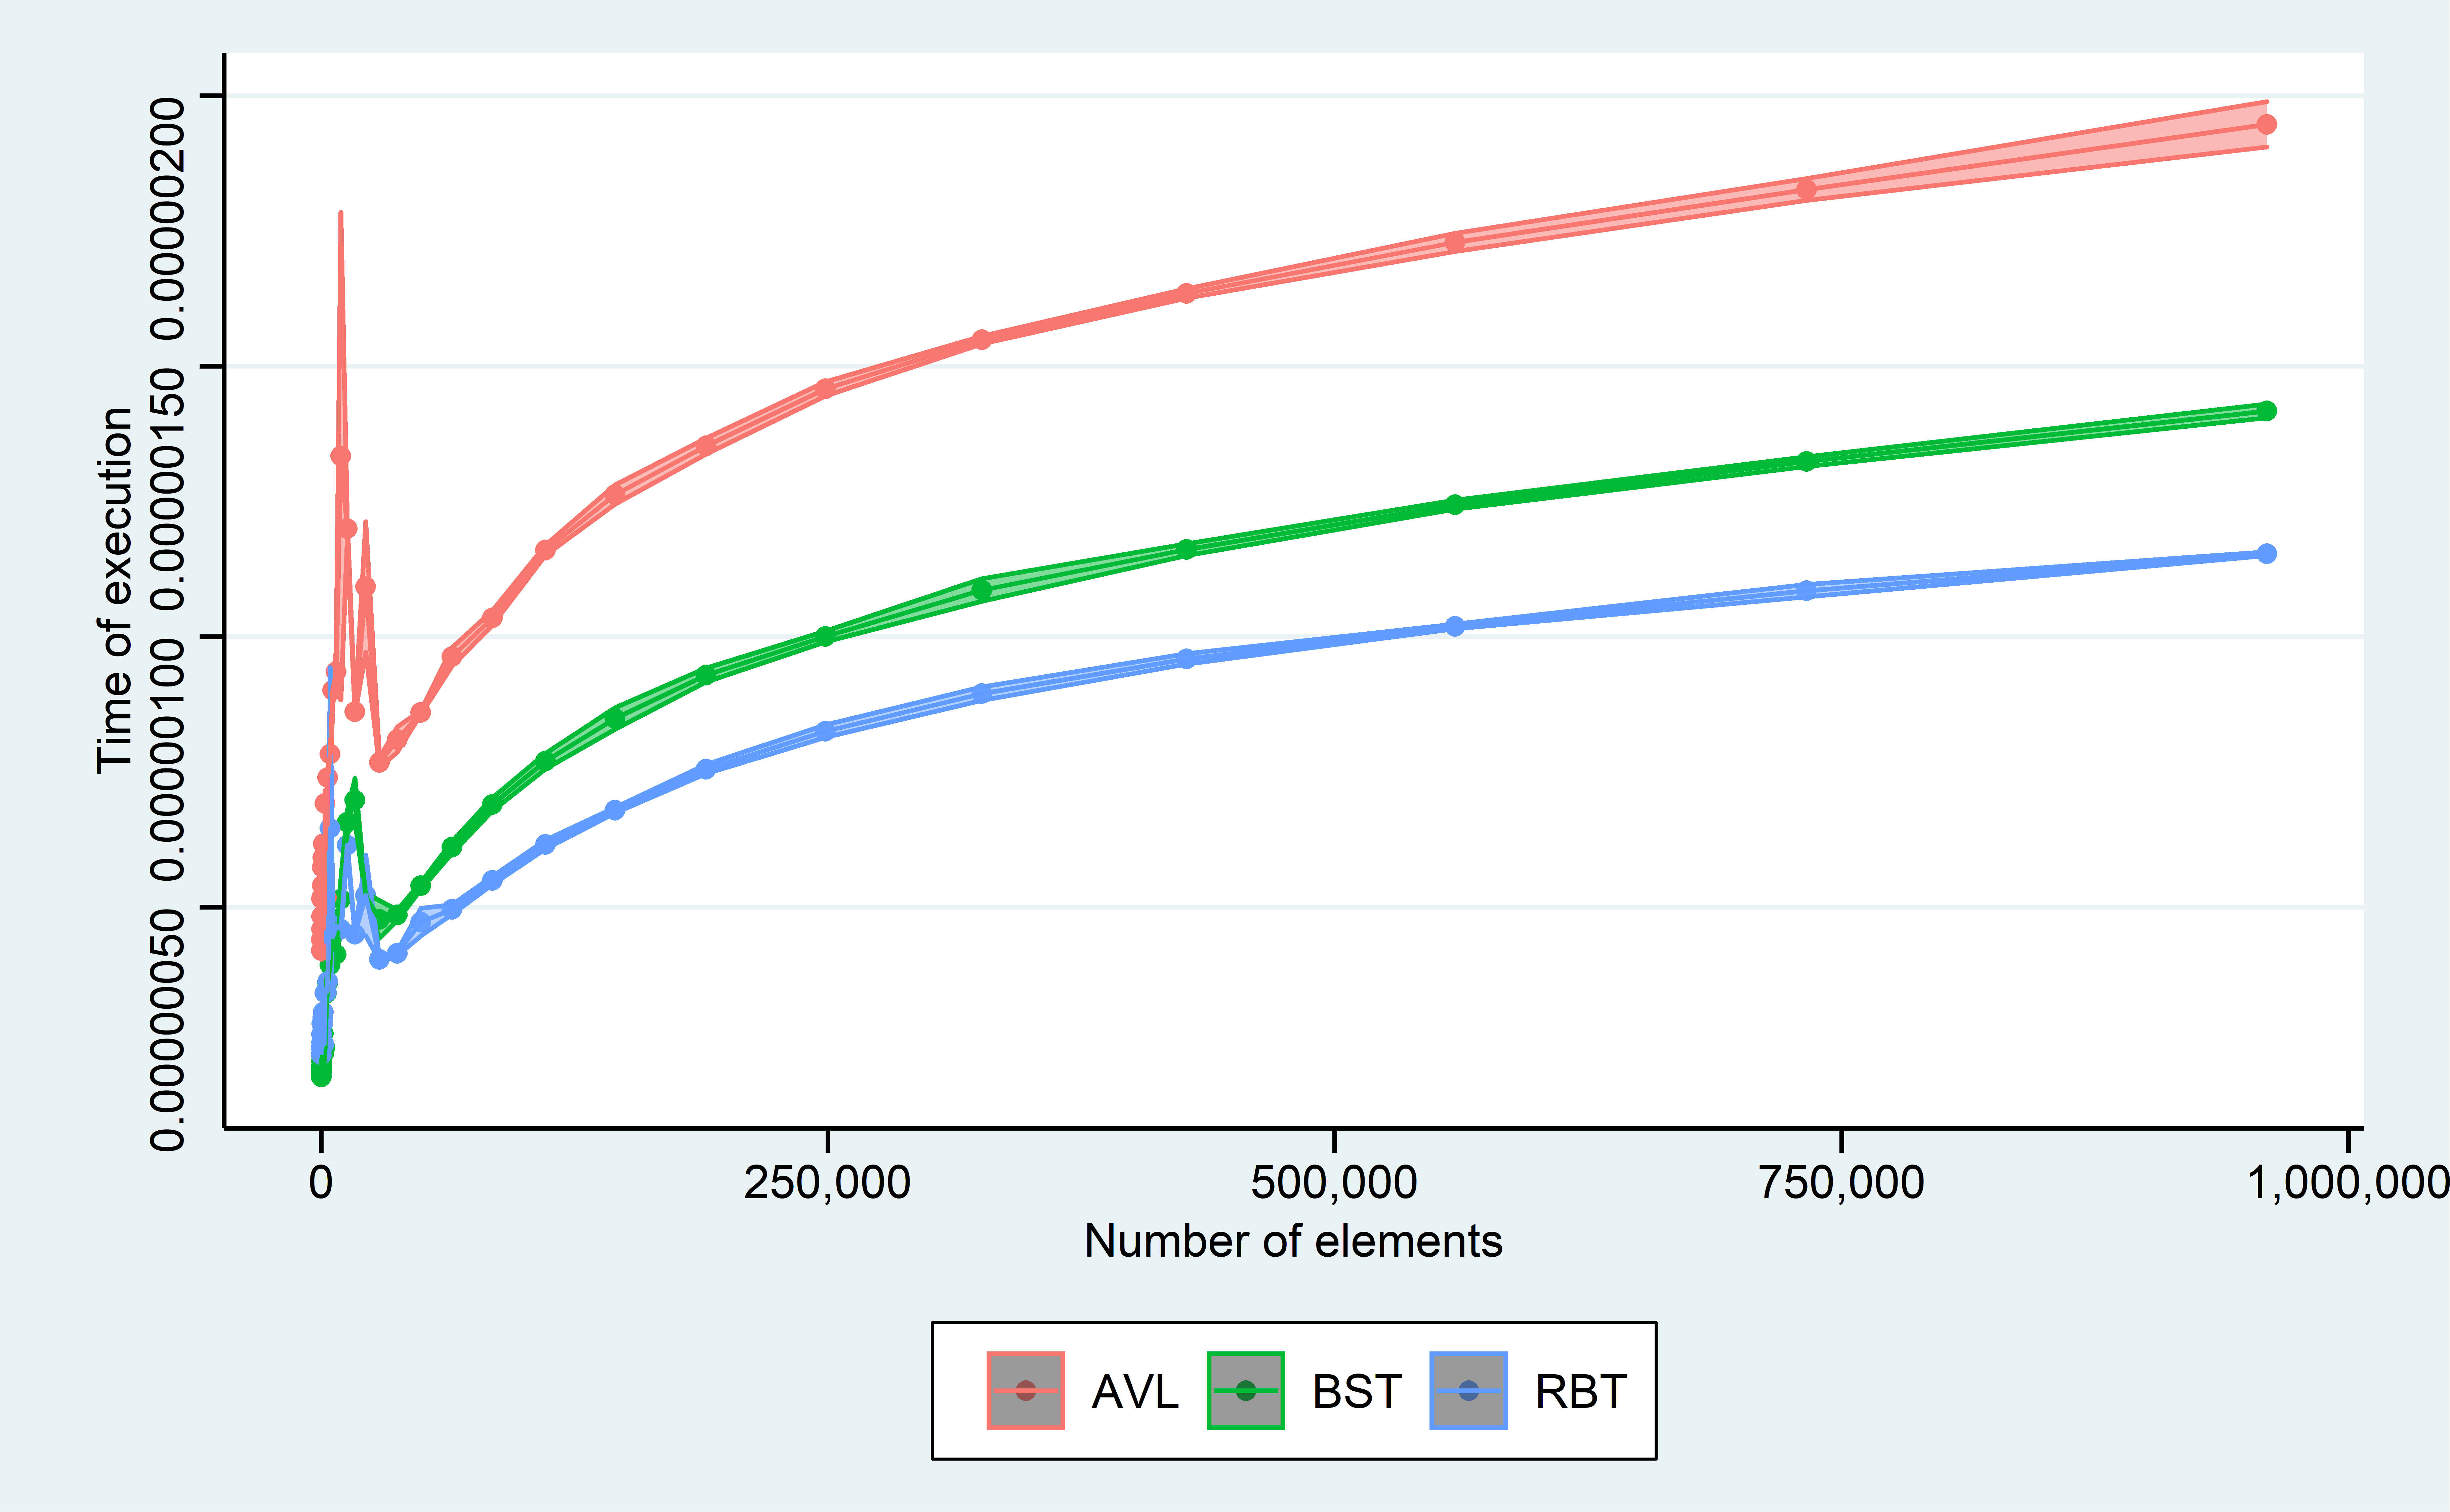
\includegraphics[width=1 \columnwidth]{Grafici/Grafico_All.png}
  		\caption{Tempo di esecuzione di $n$ operazioni di inserimento}
  		\label{fig:graph2}
	\end{figure}
	
	Le aspettative teoriche sono state principalmente rispettate. Sia i RBT che gli AVL si sono comportati come ci si aspettava.\\
	Ciò che sorprende di più è l'efficienza dei BST. Questi alberi sono, per input generati casualmente tramite l'algoritmo MT, molto efficienti in quanto non si sbilanciano. Possiamo però notare come la deviazione mediana assoluta sia molto superiore a quella degli altri due alberi, a confermare come questa efficienza sia molto legata all'input. \\
	La maggiore efficienza dei BST rispetto agli AVL può inoltre essere attribuita all'assenza, per il primo tipo di albero, di procedure di ri-bilanciamento.
	
	\newpage
	
	\subsection{Esecuzione di $n$ operazioni di inserimento con il $10\%$ di elementi ordinati}
	\label{subsection:n_op_ins_ord}
		
	\begin{figure}[h!]
		\centering
  		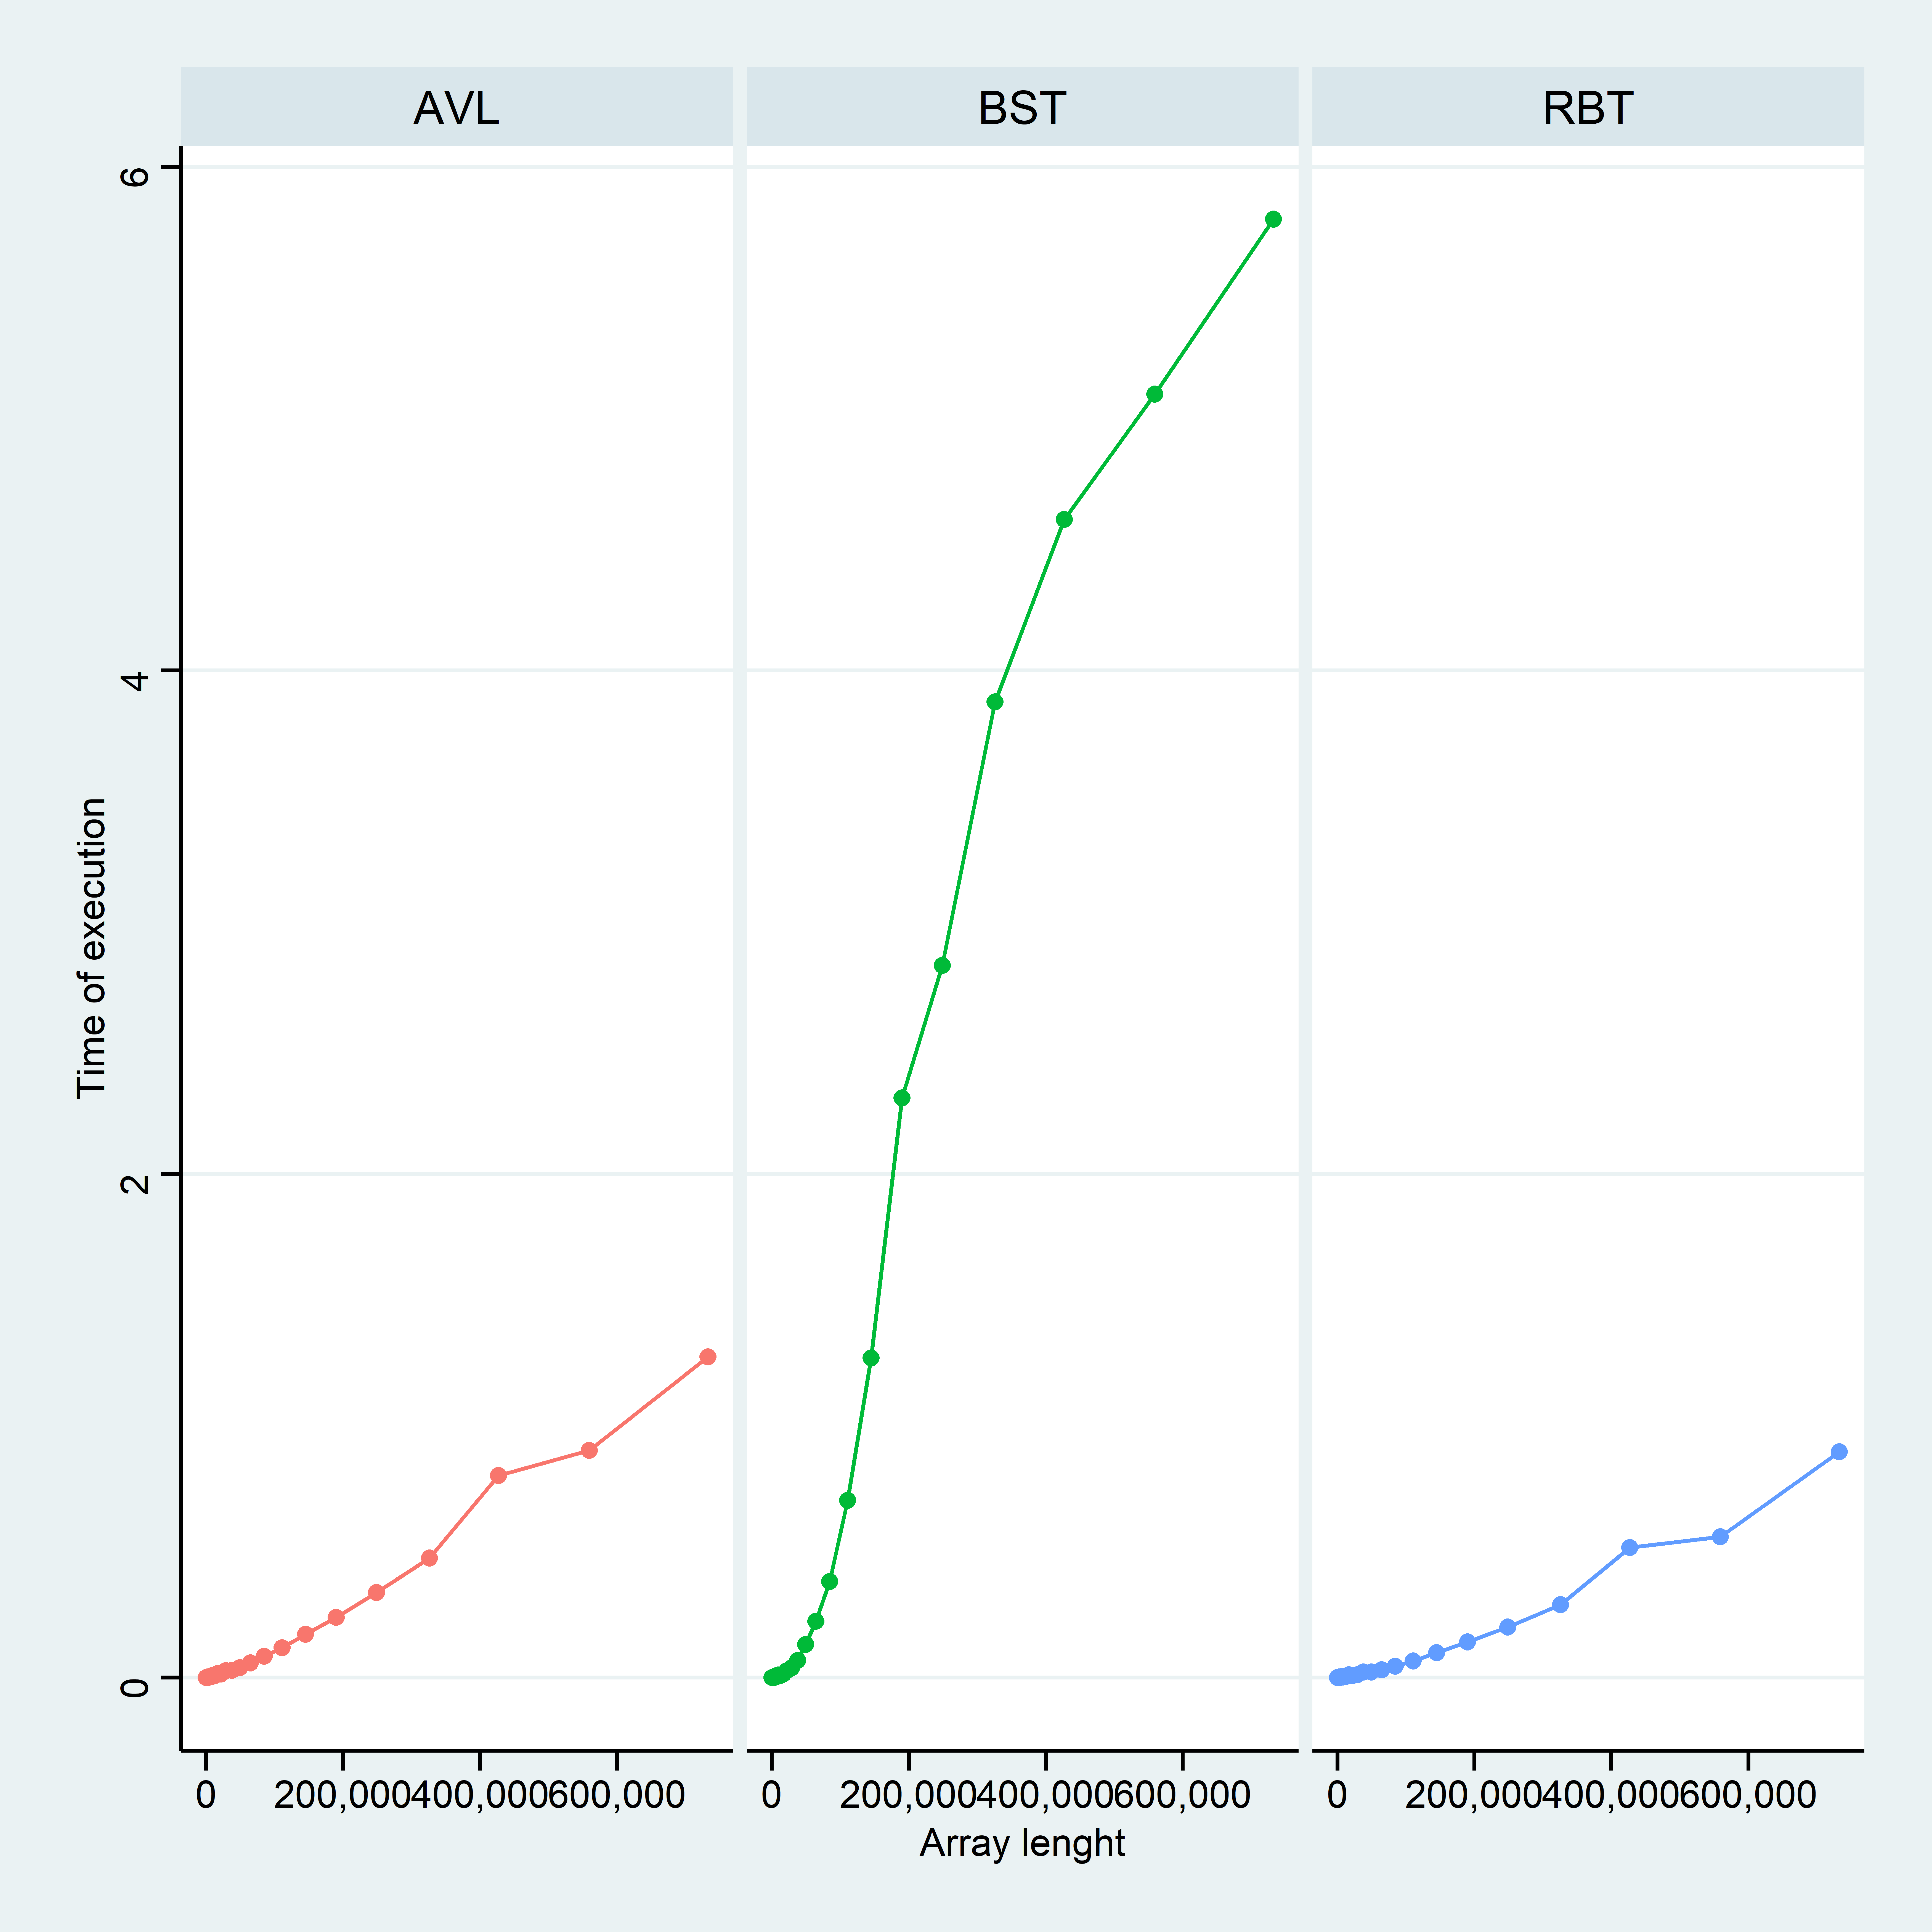
\includegraphics[width=1 \columnwidth]{Grafici/Grafico_All_ordered.png}
  		\caption{Tempo di esecuzione di $n$ operazioni di inserimento con $10\%$ di elementi ordinati}
  		\label{fig:graph2}
	\end{figure}
	
	Anche in questo grafico le aspettative teoriche sono state rispettate. Tutti gli alberi si sono comportati esattamento come predetto. \\
	Possiamo notare come i BST si siano effettivamente rivelati inefficienti rispetto agli altri due alberi. In particolare, si nota molto chiaramente l'andamento lineare nel tempo di esecuzione. \\
	Per quanto riguarda gli altri due alberi, è interessante la maggiore efficienza dei RBT rispetto agli AVL. Come predetto nella sezione \ref{par:rbt_avl}, infatti, i RBT hanno un costo di inserimento minore, dato dal funzionamento della procedura di ri-bilanciamento dell'albero stesso.
	
	\newpage
	
	\subsection{Esecuzione di $n$ operazioni di ricerca}
	\label{subsection:n_op_ric}
		
	\begin{figure}[h!]
		\centering
  		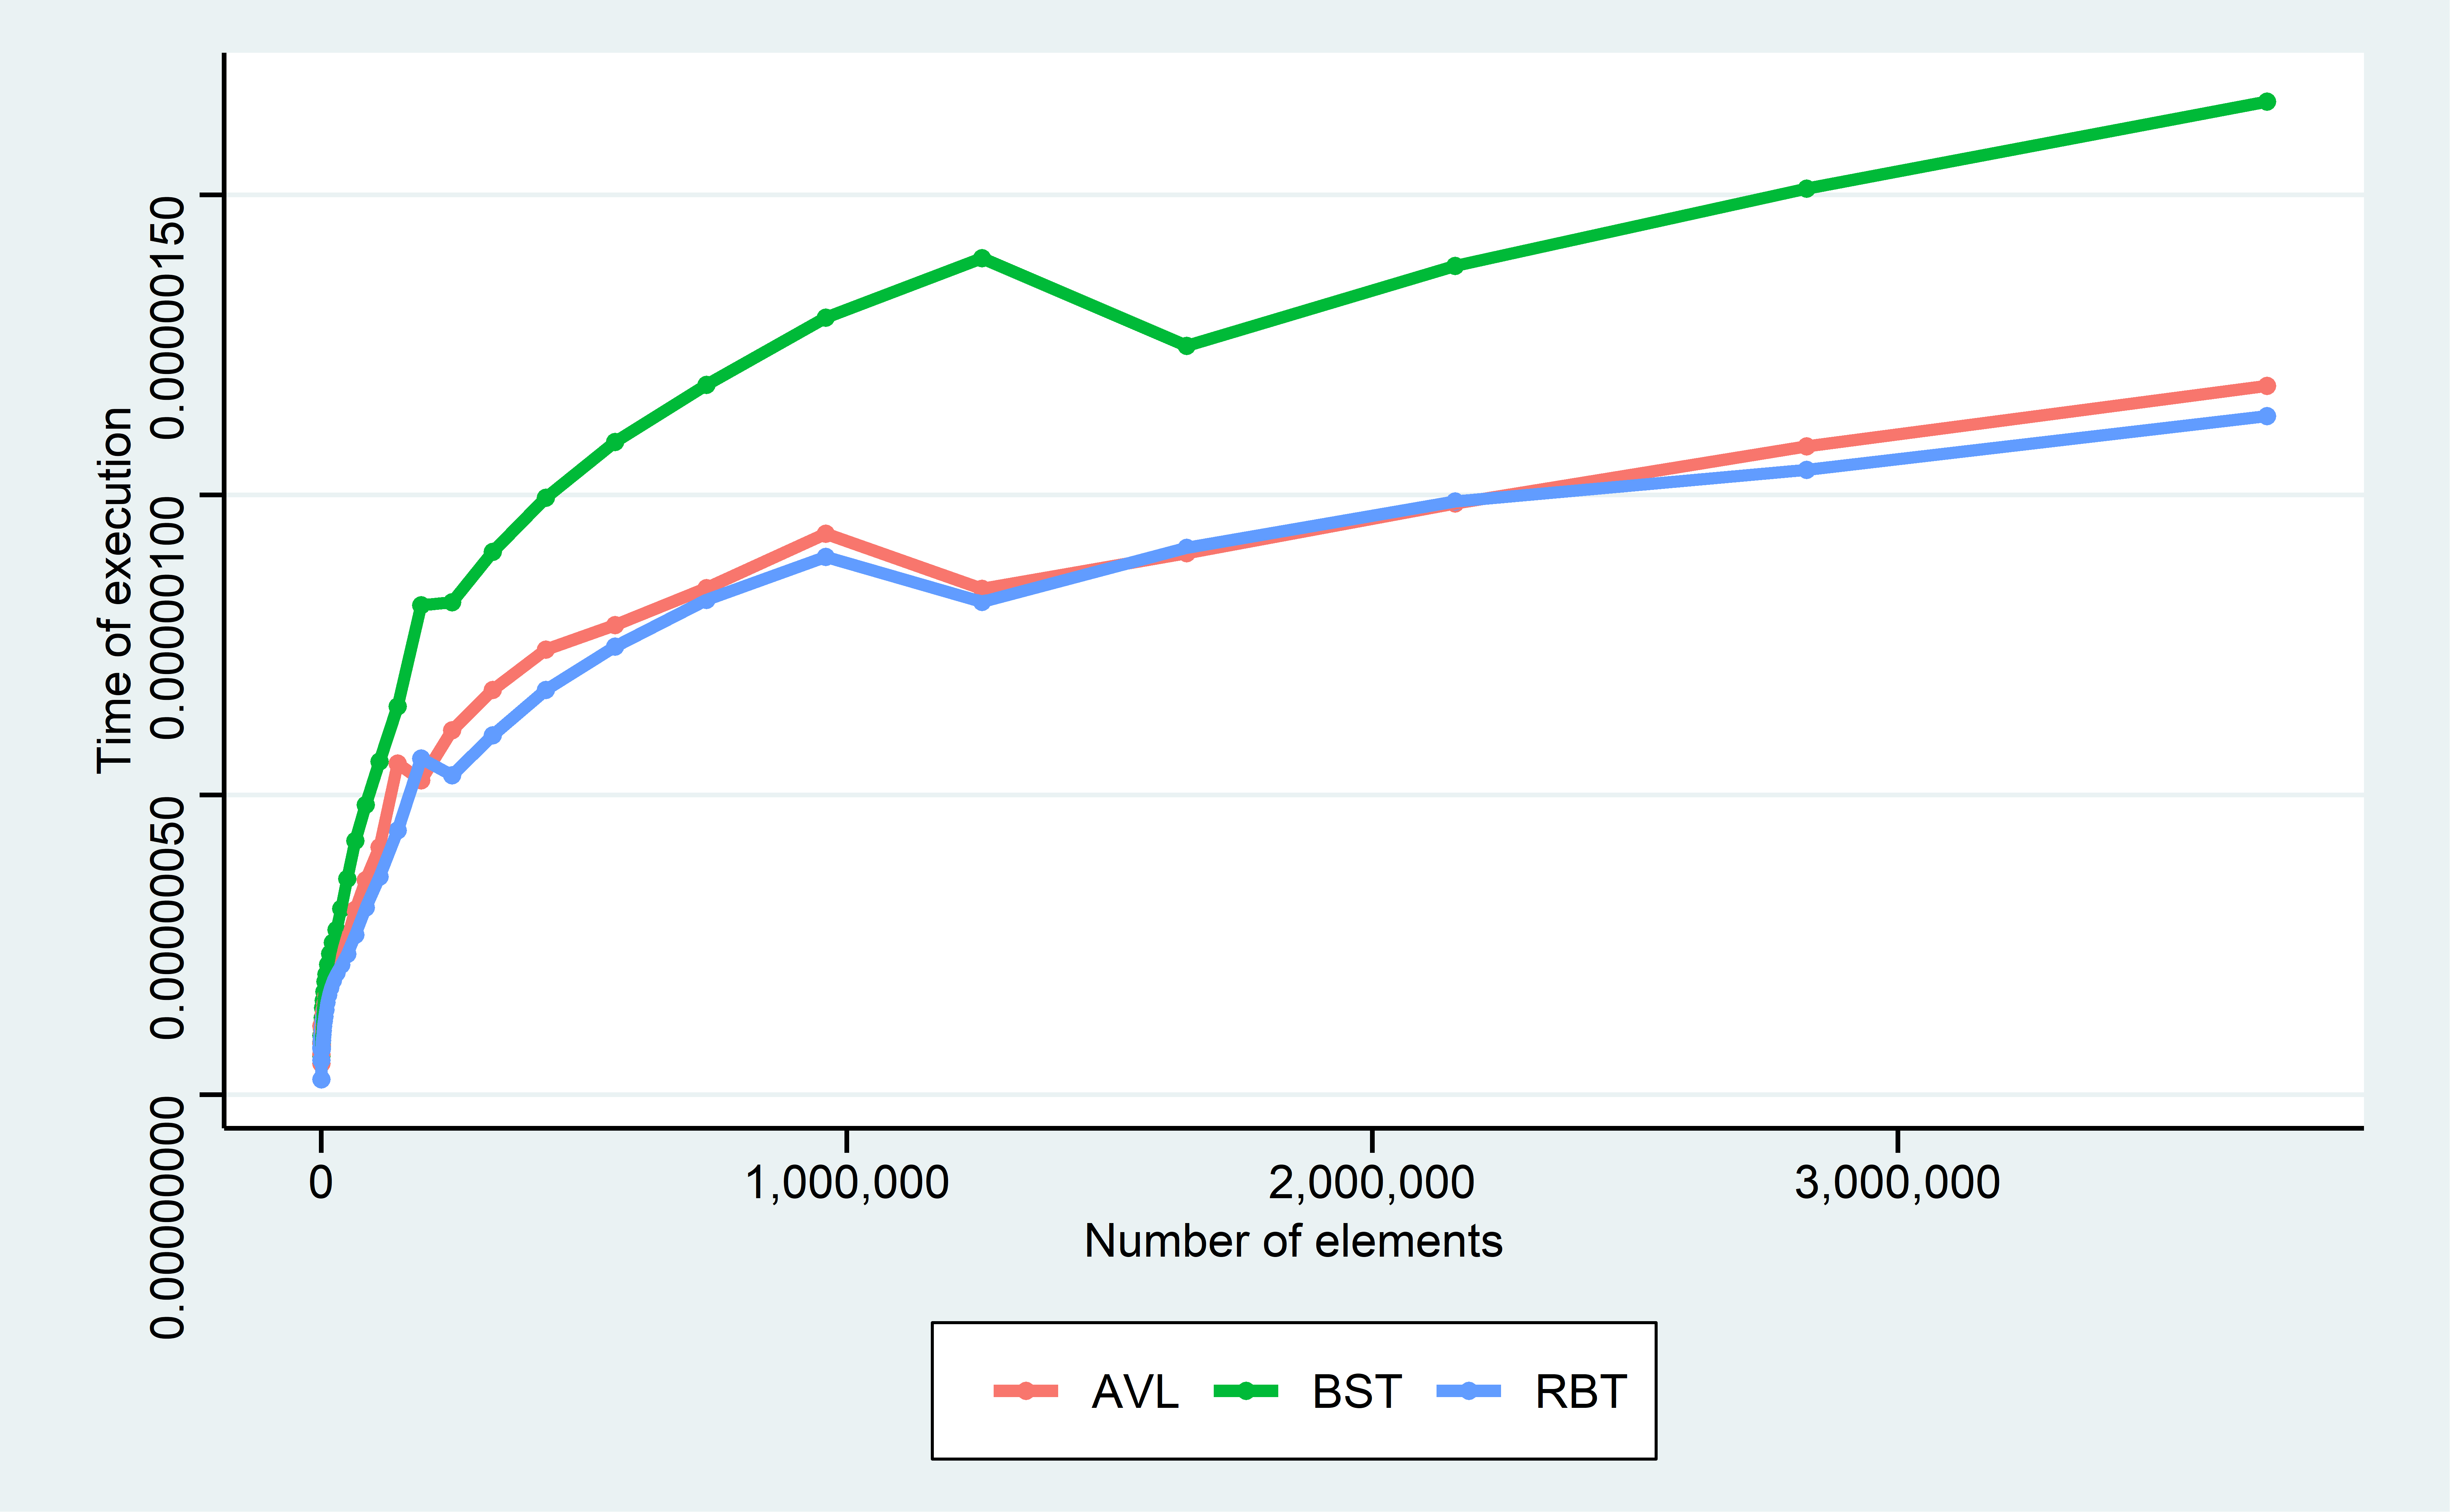
\includegraphics[width=1 \columnwidth]{Grafici/Grafico_All_finds.png}
  		\caption{Tempo di esecuzione di $n$ operazioni di ricerca}
  		\label{fig:graph3}
	\end{figure}
	
	Nel caso di sole operazioni di ricerca possiamo subito notare come i BST siano meno efficienti degli alberi AVL. Ciò è giustificato dal fatto che gli AVL sono particolarmente efficienti per le operazioni di ricerca in quanto sono effettivamente bilanciati. \\
	Risulta invece piuttosto anomala la loro minor efficienza rispetto ai RBT. Bisogna sottolineare che la differenza fra i due tempi di esecuzione è comunque minima (nell'ordine di $10^{-8}$), tuttavia questa rimane costante per svariati valori di $n$. La congettura riguardo questo anomalia riguarda l'input: essendo questo casuale è possibile che i RBT rimangano abbastanza bilanciati. Ciò tuttavia non spiega il risultato sperimentale ottenuto.
	
	\newpage
	
	\subsection{Esecuzione di $n$ operazioni di ricerca con $10\%$ di elementi ordinati}
	\label{subsection:n_op_ric}
	
	\begin{figure}[h!]
		\centering
  		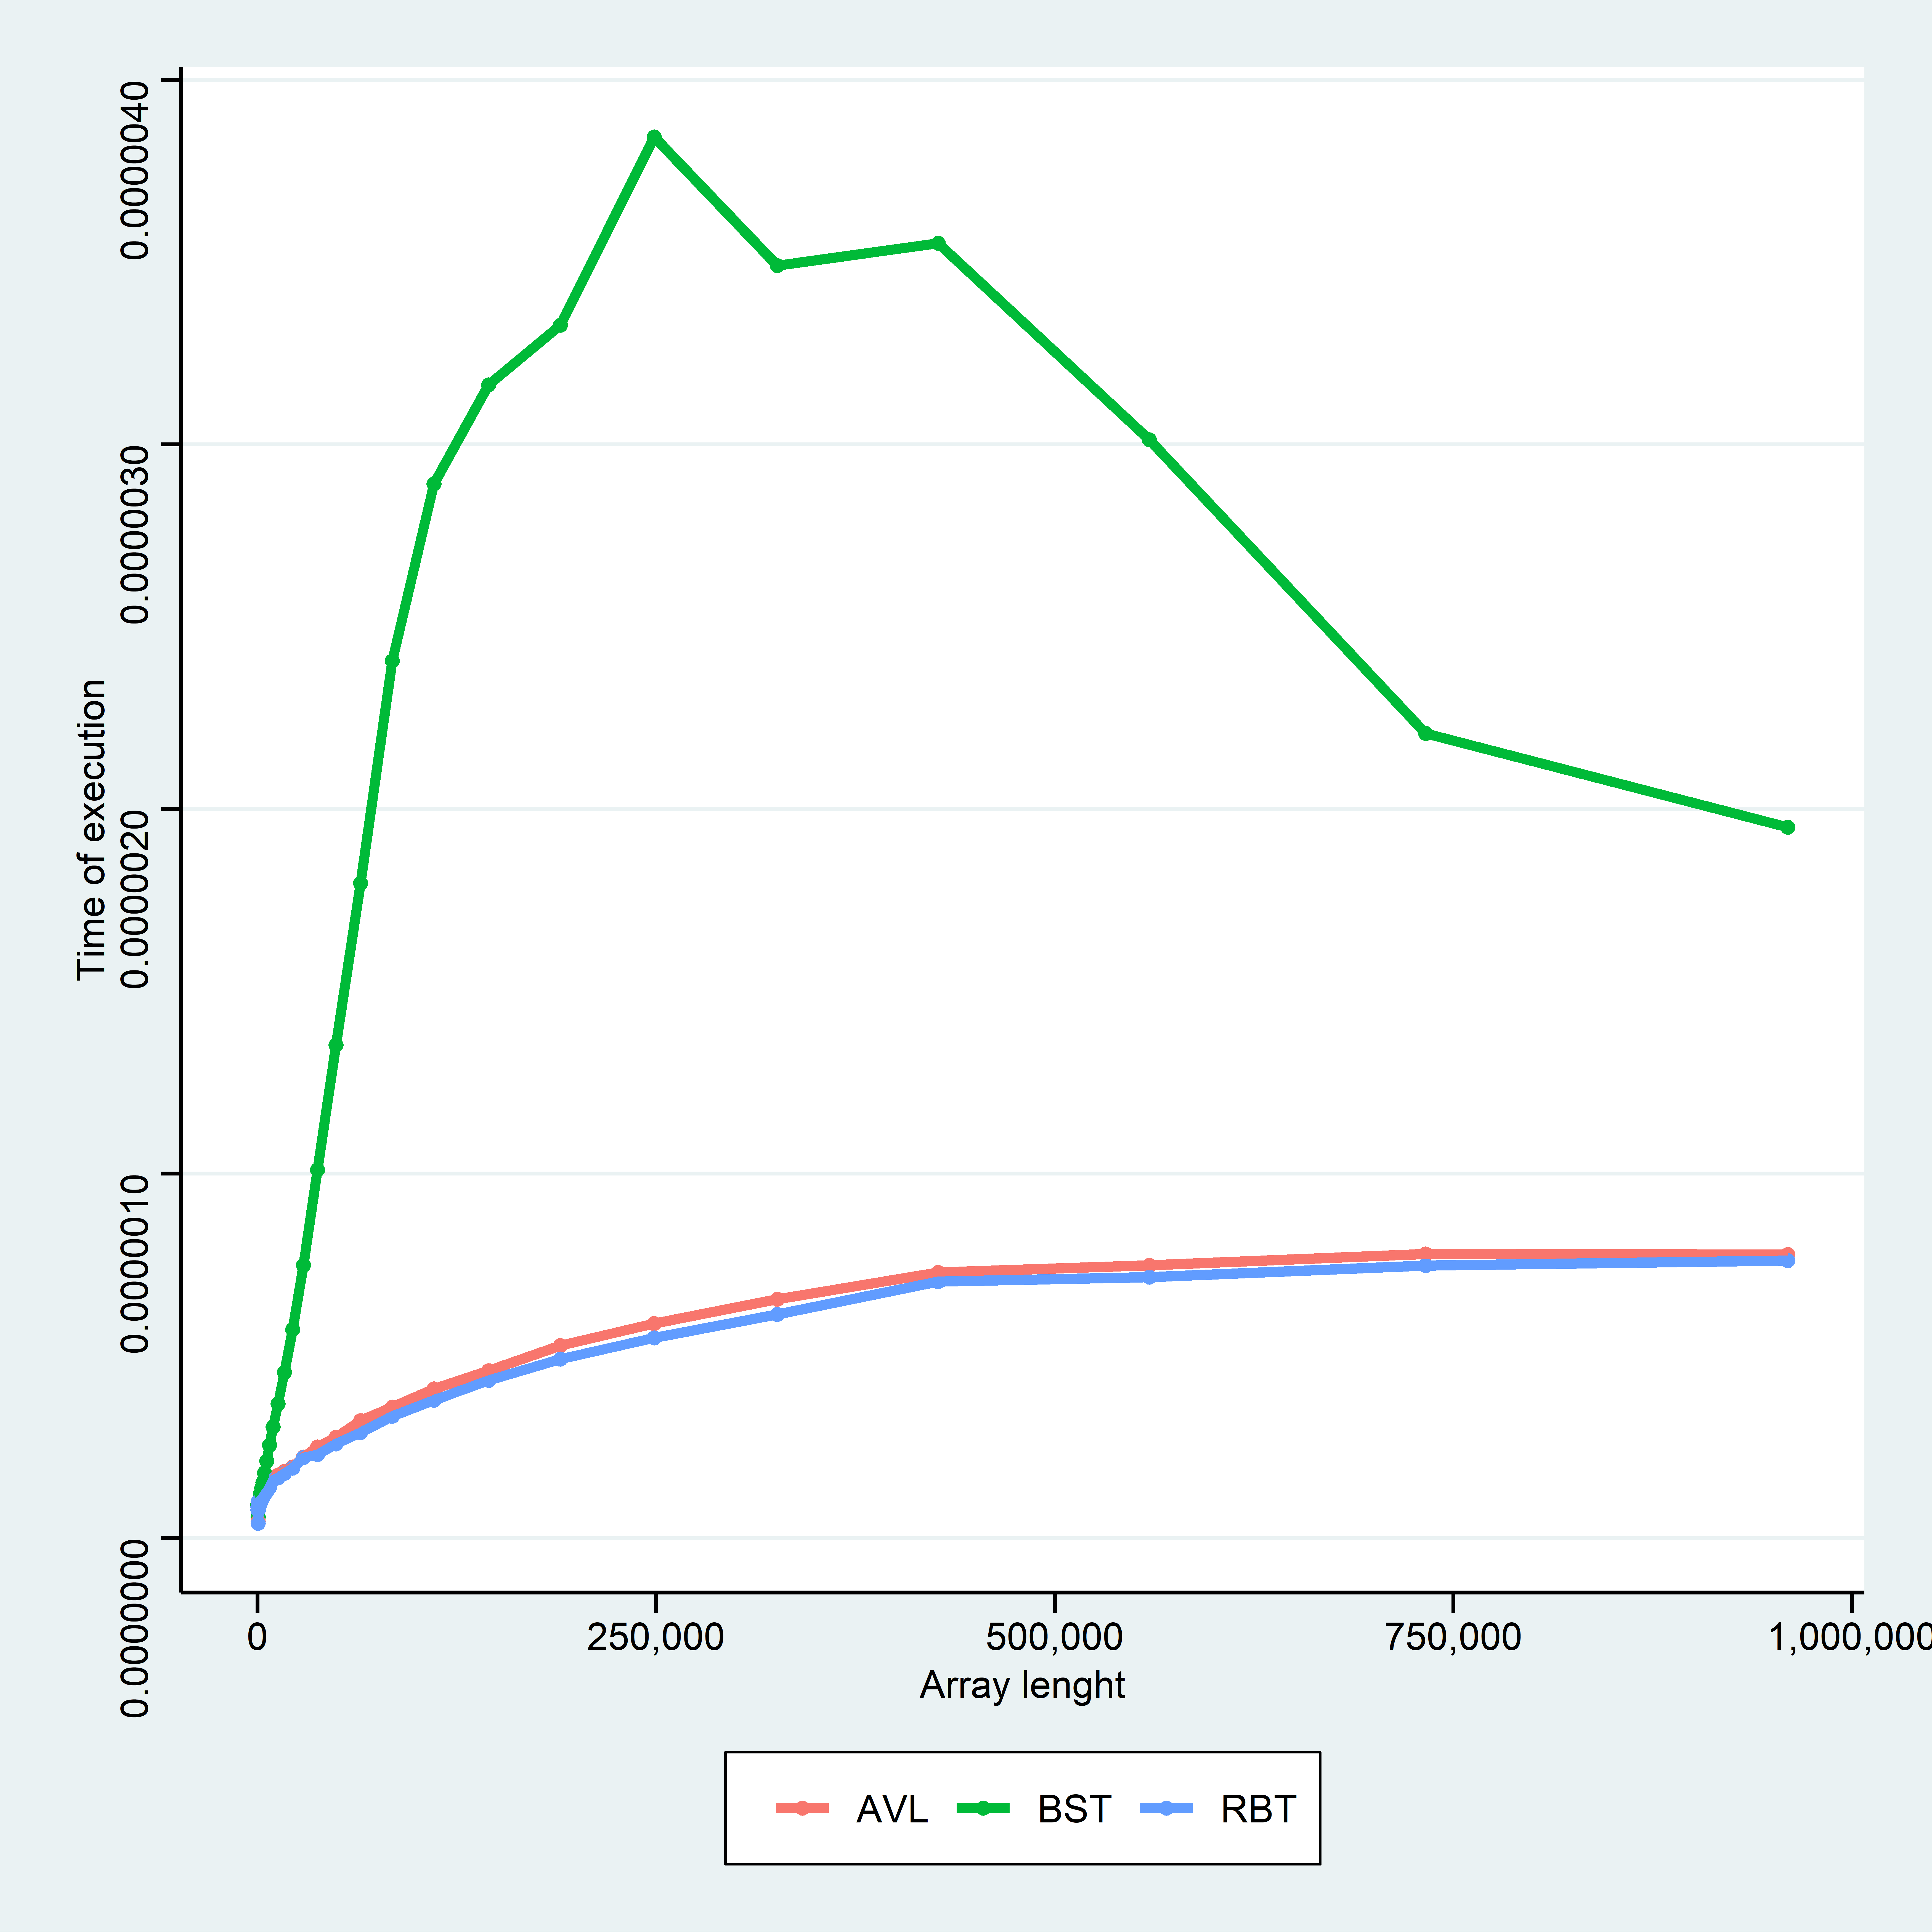
\includegraphics[width=1 \columnwidth]{Grafici/Grafico_All_find_ordered.png}
  		\caption{Tempo di esecuzione di $n$ operazioni di ricerca con $10\%$ di elementi ordinati}
  		\label{fig:graph4}
	\end{figure}
	
	Come possiamo notare, introdurre una certa quantità di elementi ordinati rende i BST estremamente meno efficienti.\\
	Gli altri due alberi invece rispecchiano lo stesso comportamento già notato nella sottosezione \ref{subsection:n_op_ric}.
	
	\newpage
	
	\subsection{Esecuzione di $n$ operazioni di ricerca con $50\%$ di elementi ordinati}
	\label{subsection:n_op_ric}
	
	\begin{figure}[h!]
		\centering
  		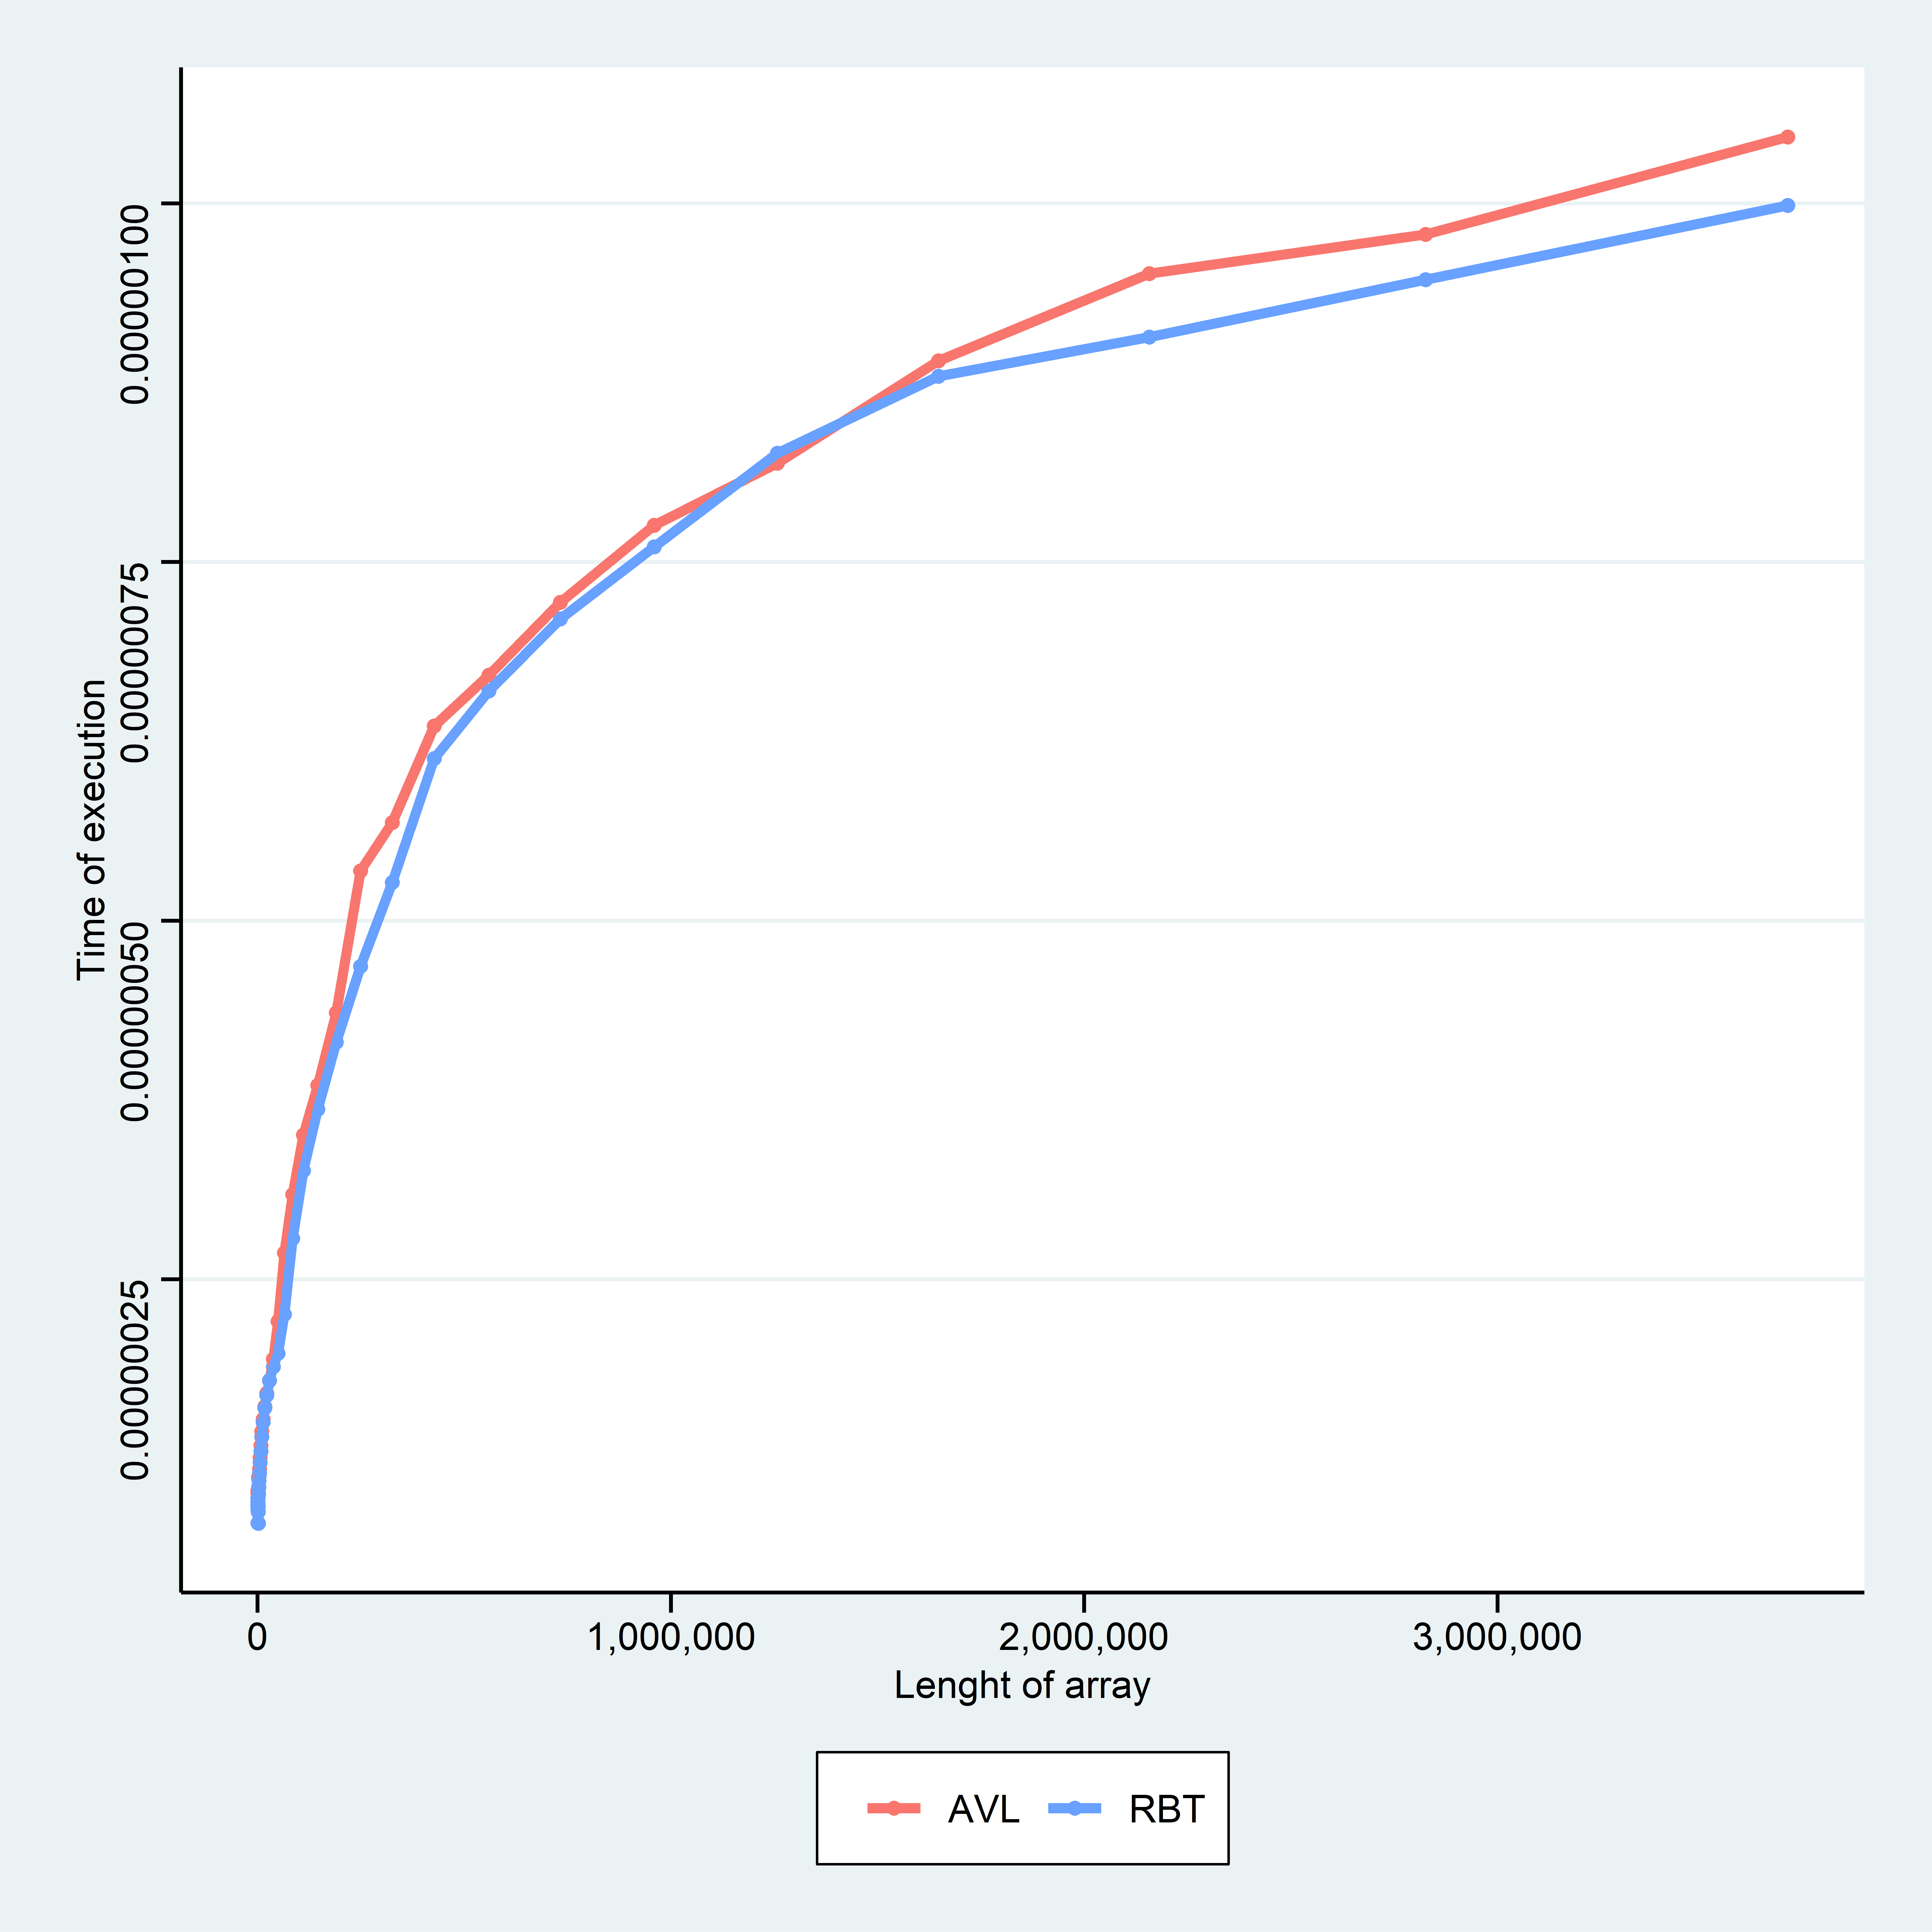
\includegraphics[width=1 \columnwidth]{Grafici/Grafico_All_find_ordered_AvlRbt.png}
  		\caption{Tempo di esecuzione di $n$ operazioni di ricerca con $50\%$ di elementi ordinati}
  		\label{fig:graph5}
	\end{figure}
	
	Un ulteriore grafico riguardante il tempo di esecuzione di operazioni di ricerca su AVL e RBT rivela come i primi possano effettivamente essere più efficienti. Questo sembrerebbe confermare la congettura precedentemente formulata nella sottosezione \ref{subsection:n_op_ric}.
	\newpage

	\section{Conclusioni}
	I risultati ottenuti sono stati molto interessanti e, sotto alcuni aspetti, inaspettati. L'analisi sperimentale degli alberi binari in questione ha certamente contribuito ad una maggior consapevolezza nell'uso degli stessi.
	\\
	Si può trarre la seguente conclusione dall'analisi sperimentale effettuata: ogni albero binario ha dei punti di forza e di debolezza. I BST sono efficienti per input casuali, anche se le loro performance tendono a deteriorare velocemente per input anche solo poco ordinati. AVL e RBT si sono rivelati entrambi molto efficienti, come previsto. In particolare, i RBT sono particolarmente efficienti nel caso di molte operazioni di inserimento, mentre gli AVL sono più efficienti per le operazioni di ricerca.\\
	
	Tutti questi sono importanti fattori di cui tenere conto nell'implementare in maniera efficiente degli alberi binari.
	
\end{document}
